
\section*{Ejercicios}

\begin{itemize}
    \item Identificar\\
        ¿Que hacen los siguientes diagramas de flujo?
          \begin{center}
            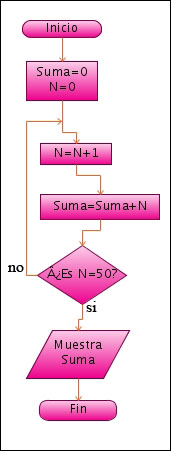
\includegraphics[scale=0.5]{Imagenes/image11}.
            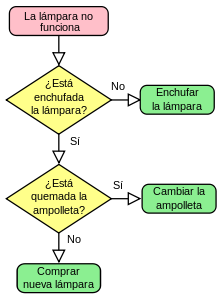
\includegraphics[scale=0.8]{Imagenes/image03}
          \end{center}

    \item Volviendo a sumar\\
        Una progresión aritmética consiste en calcular la suma de números consecutivos. Por ejemplo, la suma de los primeros números naturales hasta $n$ es:
        $1 + 2 + 3 + ... + n = \Sigma_{1\leq i\leq n}i$
        
        \newpage
    \item Linea de producción \\
        En la empresa BoxDrop S.A. se tiene una banda transportadora en la cual se mueven 3 tipos de caja. Cada caja tiene un color distintivo que indica su destino. Las cajas azules son repuestos para los talleres subsidiarios, las cajas amarillas contienen formularios de impuestos e información contable y las cajas rojas son objetos frágiles. Un operador debe tomar cada caja de la banda transportadora y depositarla en los contenedores que las enviarán a su destino final. \\
        Construya un diagrama de flujo para modelar el trabajo del operador al clasificar N cajas.

        
        \newpage
        
\end{itemize}


